\chapter{背景知識}

\section{國際化}
國際化(Internationalization)\cite{internationalization},簡寫為i18n,其中18代表i和n之間的18個英文字母。國際化是開發軟體時,將軟體本身和特定語言、地區脫鉤的一個過程,除了可以滿足不同的地區、文化的大眾需求,移植軟體到不同的語言環境時,也不須改變內部程式的實作。

\section{自動化驗收測試}
驗收測試(Acceptance Testing)\cite{se},是一種站在使用者的立場,去檢驗一個真實存在的系統,是否滿足使用者需求與預期的測試方法。

而透過撰寫自動化測試腳本\cite{AT},如今我們可以執行更符合成本,且更加精確的自動化驗收測試。改善了過往手動執行驗收測試時,存在的人為操作誤差、系統問題無法即時呈現、成本較高等問題。
\section{Robot Framework}
Robot Framework\cite{rf}\cite{rfguide}是一個開源的框架語言,可以用來執行自動化驗收測試或機器人自動化,核心框架是由Python\cite{python}編寫而成,測試者可以使用Python或Java擴充其函式庫。其特色是擁有簡單的語法,以及容易理解的原生關鍵字(Keyword),測試者可以視需求使用並包裝成更接近自然語言的關鍵字。

\subsection{Robot Framework測試腳本}
一個Robot Framework 的測試腳本基本上由三個區塊構成,分別是:
\begin{itemize}
    \item[1.]Settings: 包含了使用到的library與resource file,也可以將Test Setup(測試腳本執行前要做的動作)、Test Teardown(測試腳本執行後要做的動作)定義於此。
    \item[2.]Test Cases: 在此測試者可以為各項想要驗證的使用者需求,撰寫核心的測試腳本
    \item[3.]Keywords: 如果測試腳本使用並非Robot Framework的原生關鍵字,或未被定義於其他resource file中,測試者可以在此處撰寫出新的關鍵字去達到測試目的。
\end{itemize}

\subsection{Robot Framework測試報表}
在測試腳本運行結束後,Robot Framework會產生出一份測試報表,記錄了整體的執行狀況,包含測試通過或失敗、腳本執行時間,並透過可展開的階層式圖表,方便測試者去追蹤到當前出現問題的關鍵字,進而修復錯誤。

\section{XPath}
XPath\cite{xpath},全名為 XML Path Language,可以用來定位XML檔案中某節點所處在的位置。在使用Robot Framework撰寫的網頁自動化驗收測試中,我們便時常需要藉助XPath,去找到並確定畫面上某元件的位置,以對其狀態進行測試。

\section{第一版i18n的系統架構與運作原理}
\begin{figure}[H]
    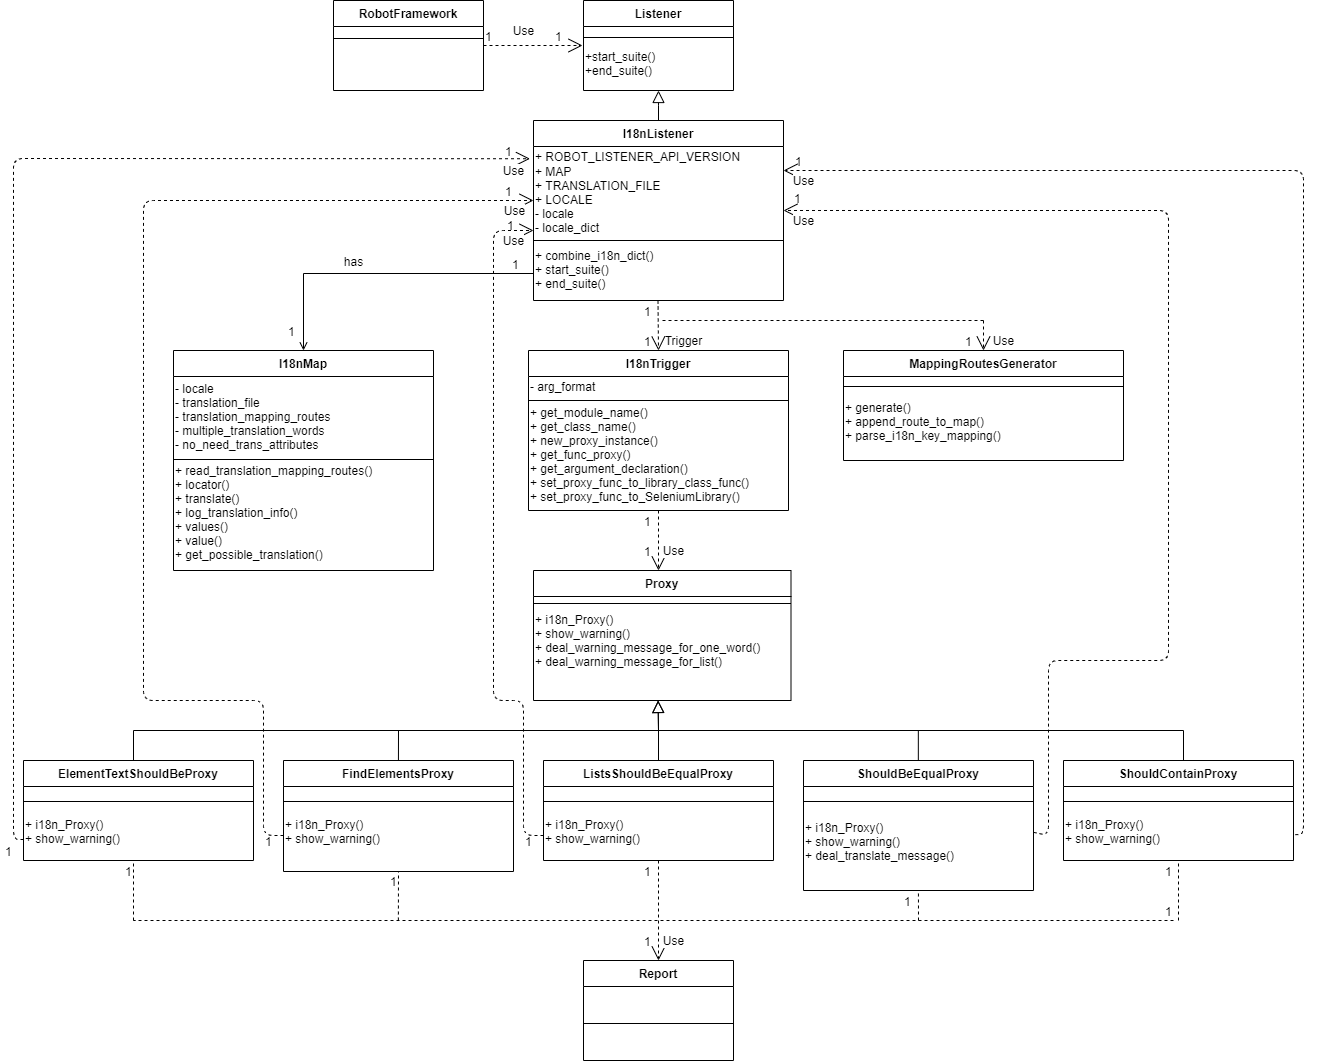
\includegraphics[width= 1.1\textwidth]{../UML/i18n class diagram-第一版i18n class diagram.png}
    \caption{第一版i18n的系統類別圖}
    \label{1stI18nClassDiagram}
\end{figure}
第一版i18n的系統類別圖(如圖~\ref{1stI18nClassDiagram}),包含了3個 Robot Framework原生類別: RobotFramework、Listener、和Report;第一版i18n所設計的5個系統類別 :I18nListener、MappingRoutesGenerator、I18nMap、I18nTrigger、Proxy,以及5個實作自Proxy\cite{proxy}類別的代理關鍵字類別: ShouldContainProxy、ElementTextShouldBeProxy、FindElementProxy、ListsShouldBeEqualProxy、ShouldBeEqualProxy。\cite{i18n}

I18nListener類別實作Listener類別,負責程式開始與結束時執行start\_suite()和end\_suite()的內容,並對MappingRoutesGenerator、I18nMap、I18nTrigger三個類別進行初始化的動作。I18nMap類別負責處理各個代理關鍵字類別透過I18nListener類別的呼叫,並將待翻譯詞做翻譯後回傳。I18nTrigger類別透過new\_proxy\_instance()函式建立各個代理關鍵字類別的實例;並使用set\_proxy\_func\_to\_library\_class\_func()、set\_proxy\_func\_to\_SeleniumLibrary()兩函式,將代理關鍵字類別的實作包裝於Robot Framework原生關鍵字之外,使每次呼叫關鍵字時,必先執行代理關鍵字的實作。MappingRoutesGenerator類別負責以英文JSON翻譯檔為基準,產生出翻譯路徑檔,讓測試腳本運行在其他語言環境下,可以根據此路徑,在所屬語言的JSON翻譯檔下找到正確的翻譯。Proxy類別提供了一個介面,讓實作Proxy類別的代理關鍵字類別可以根據各自的需要,去擴充內部的實作;其中,i18n\_Proxy()函式提供各代理關鍵字類別撰寫核心的功能。

\begin{figure}[H]
    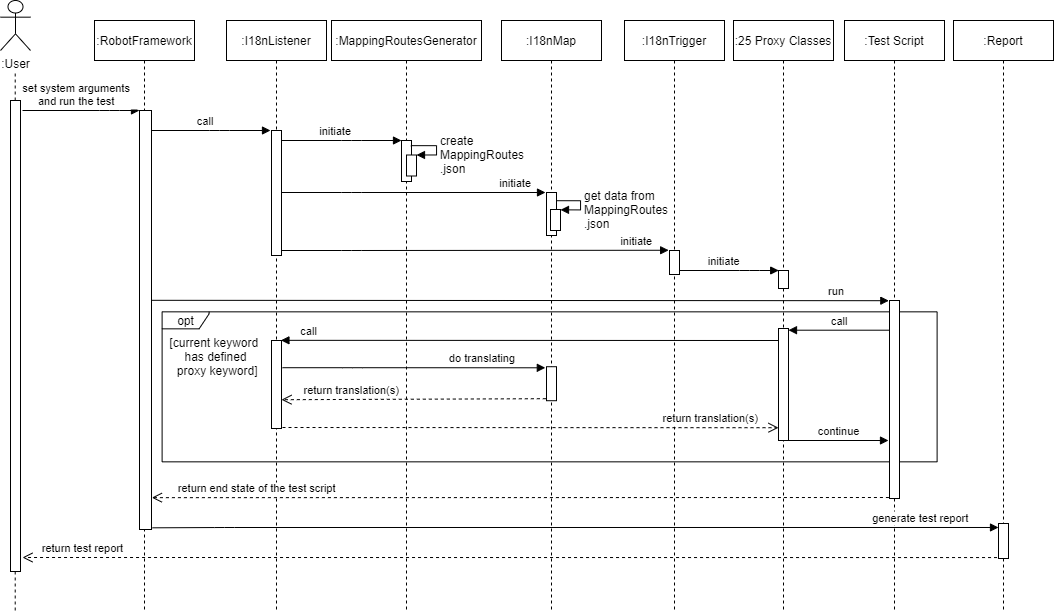
\includegraphics[width= 1.1\textwidth]{../UML/i18n sequence diagram-第一版i18n系統流程.png}
    \caption{第一版i18n的系統流程Sequence Diagram}
    \label{1stI18nSequenceDiagram}
\end{figure}
系統流程的部分(如圖~\ref{1stI18nSequenceDiagram}),在使用i18n工具執行測試腳本前,使用者必須於Red編輯器\cite{red}中的Additional Robot Framework arguments設定系統參數為-d out –L debug -–listener i18n/listeners/I18nListener.py:zh-TW,zh-TW代表當前語言為繁體中文-台灣(如圖~\ref{rfSysArgsSetting})。

\begin{figure}[H]
    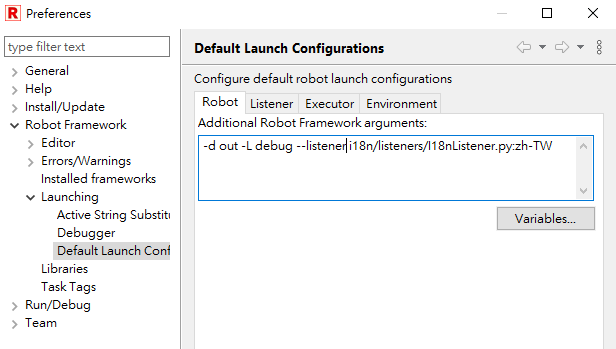
\includegraphics[width= 1.1\textwidth]{../論文截圖/3-1-3-1 設定系統參數.png}
    \caption{Robot Framework系統參數設定}
    \label{rfSysArgsSetting}
\end{figure}
測試執行時,系統會先去呼叫I18nListener類別並執行其實作。之後初始化MappingRoutesGenerator類別,藉由讀取由使用者自行提供的JSON格式翻譯檔(如圖~\ref{英文的JSON格式翻譯檔示例}),建立出一份由「待翻譯詞」和「Key階層」構成的翻譯路徑檔(如圖~\ref{翻譯路徑檔});例如待翻譯詞‘Support’,有兩種Key階層的路徑: "['SUPPORT']" 和 "['SUB\_BAR']['BLUE\_TITLE']['MICROSOFT\_SUPPORT']",代表‘Support’在多國語言網頁中,會在不同情境下被翻譯成兩種不同的詞彙。接著系統會依序初始化I18nMap、I18nTrigger,以及所有代理關鍵字類別。

當執行完上述工作後,測試腳本才會正式開始執行;每當腳本運行到一個有定義代理的關鍵字,系統就會去呼叫對應的代理關鍵字物件,並執行翻譯邏輯。最後,當測試腳本執行結束,系統則會將一詞多譯的warning資訊顯示在報表上。

\begin{figure}[H]
    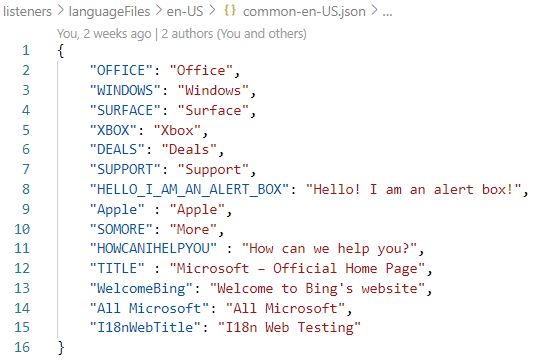
\includegraphics[width= 1.1\textwidth]{../論文截圖/3-1-3-2 JSON格式翻譯檔.png}
    \caption{英文的JSON格式翻譯檔示例}
    \label{英文的JSON格式翻譯檔示例}
\end{figure}

\begin{figure}[H]
    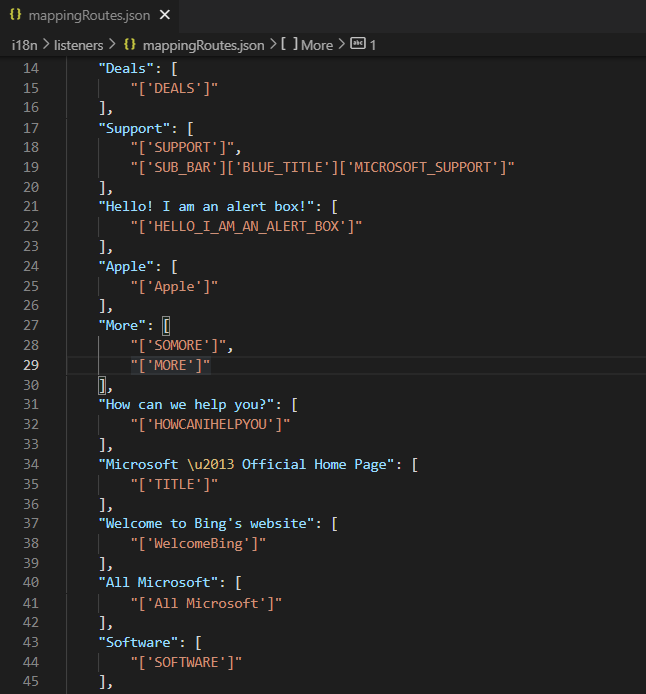
\includegraphics[width= 1.1\textwidth]{../論文截圖/3-1-3-3 翻譯路徑檔.png}
    \caption{翻譯路徑檔部分示例}
    \label{翻譯路徑檔}
\end{figure}
